\section{Particle Injection Chain} \label{sec:lhc:injection}

\begin{figure}[!htbp] 
  \begin{center}
    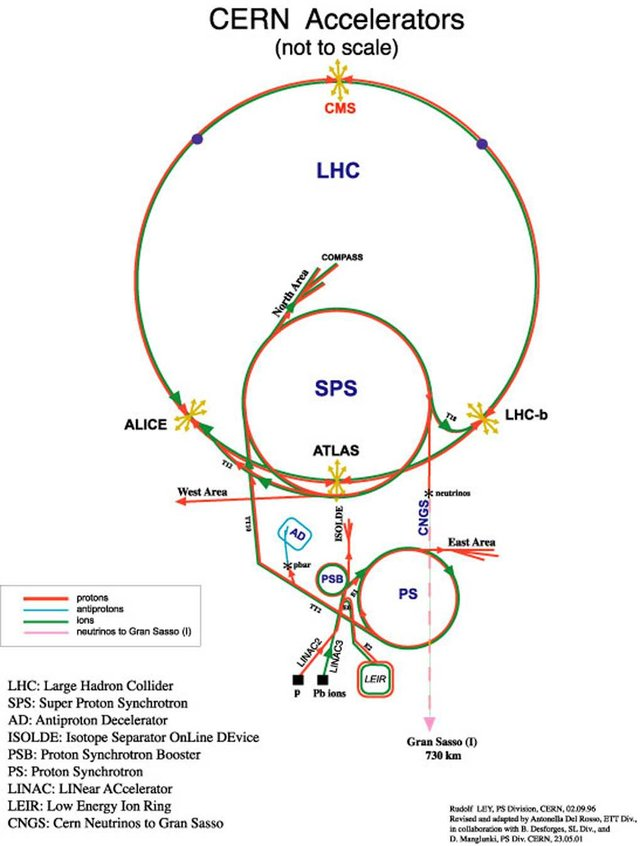
\includegraphics[width=\linewidth]{figures/lhc/injection.jpg}
    \caption{ Sketch of the  CERN accelerator complex \cite{Servicegraphique:1708849}.} 
    \label{fig:injection_chain} 
  \end{center} 
\end{figure}

We begin with the most common element in the Universe, hydrogen, as the source
of protons.  A bottle of hydrogen gas provides 100 microsecond pulses of raw
$H_{2}$ which is then injected into a Duoplasmatron \cite{Scrivens:1382102}.
There,  a strong electric field and free electrons from a cathode ionize the
molecule into bare $H^{+}$ - a proton!  These protons are then accelerated by
a 90 kV electric field, leaving the Duoplasmatron at 1.4\% the speed of light
($\sim$4000 km/s) or, in particle physics units, $\sim 90~\keV$
\cite{duoplasmatron_doc}. The bare protons are then fed into the accelerating
Radio Frequency (RF) cavities of Linear Accelerator 2 (LINAC2).  Inside,
conductors charged by a powerful oscillating electromagnetic field accelerate
the protons to an energy of $50~\MeV$. Along the way, small quadrupole magnets
shape the proton bunch to ensure they remain in a tight beam.  This pattern of
acceleration with RF cavities and shaping/tuning with magnets is then repeated
with CERN's first synchrotron, the Proton Synchrotron (PS), rendering a $1.4~\GeV$
proton beam.  The final step before the LHC comes with the Super Proton
Synchrotron where the same technologies are implemented to produce $450~\GeV$
protons, ready for injection into the LHC. A diagrammatic representation of
this chain can be seen in \Cref{fig:injection_chain}. 

In order to produce proton-proton collisions, the LHC uses two beams
circulating in opposite directions.  The beams are not continuous, but instead
consist of bunches of around 120 billion protons with a spacing of 25 ns.
The LHC circumference allows for 3564 bunches, however only 2808 are
filled per beam due to safety requirements and injection limitations.  Each
beam takes 4 minutes and 20 seconds to fill and then 20 additional minutes
for the protons to reach their maximum energy of $7~\TeV$, or
$99.99999991\%$ the speed of light! Under normal operating conditions these
beams can be used for 8 to 10 hours.
